56. $\cfrac{(x^2-9)(y-x+1)}{x-3}=0\Leftrightarrow\begin{cases} \left[\begin{array}{l}x=3,\\ x=-3,\\ y=x-1.\end{array}
ight.\\ x
eq3.\end{cases}$
$$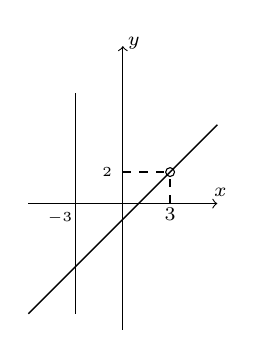
\begin{tikzpicture}[scale=0.2]
\tikzset {line01/.style={line width =0.5pt}}
\tikzset{line02/.style={line width =1pt}}
\tikzset{line03/.style={dashed,line width =0.5pt}}
%\filldraw [black] (0,0) circle (1pt);
\draw [->] (-6,0) -- (6,0);
\draw [->] (0,-8) -- (0,10);
\draw[line01] (-6,-7) -- (6,5);
\draw[line01] (-3,-7) -- (-3,7);
\draw[line03] (3,0) -- (3,2);
\draw[line03] (0,2) -- (3,2);
%\draw[line03] (0,-2) -- (1,-2);
\draw (6.2,0.7) node {\scriptsize $x$};
%\draw (-1.2,-2) node {\scriptsize $-2$};
%\draw (-0.7,2) node {\scriptsize $2$};
%\draw (-0.7,1.2) node {\scriptsize $1$};
\draw (-1,2) node {\tiny $2$};
\draw (3,-0.7) node {\scriptsize $3$};
\draw (-4,-0.9) node {\tiny $-3$};
\draw (0.7,10.2) node {\scriptsize $y$};
\draw (3,2) circle (8pt);
%\draw (-2,-3) circle (8pt);
\end{tikzpicture}$$
